\chapter{System Testing}
System testing is testing conducted on a complete integrated system to evaluate the system's compliance with its specified requirements. System testing takes, as its input, all of the integrated components that have passed integration testing.

\begin{figure}[H]
    \centering
    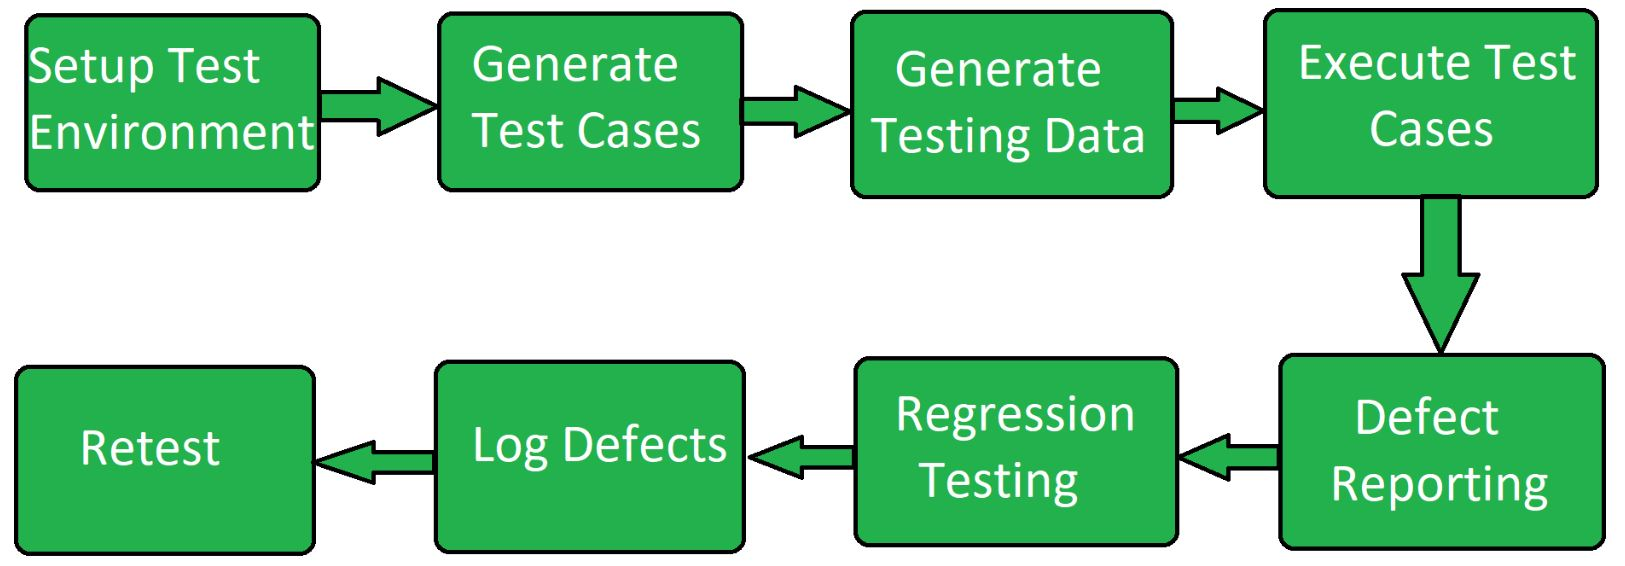
\includegraphics[width=\textwidth]{testing}
    \caption{System Testing Process}
    \label{fig:testing_process}
\end{figure}

\section{Types of System Testing}
\begin{itemize}
 \item Performance Testing
 \item Load Testing
 \item Stress Testing
 \item Scalability Testing
\end{itemize}
\clearpage

\section{Our System Tests and Results}

\begin{table}[H]
    \centering
    \begin{tabular}{|l|l|l|c|} \hline
        Test Case & Expectation & Reality & Result \\\hline\hline
        Username invalid & Registration fails & Registration fails & Passed \\\hline
        Password invalid & Registration fails & Registration fails & Passed \\\hline
        Server invalid & Registration fails & Registration fails & Passed \\\hline
        Credentials not given & Does not register & Does not register & Passed \\\hline
        Server not given & Does not register & Does not register & Passed \\\hline
        Server offline & Registration timeout & Registration timeout & Passed \\\hline
    \end{tabular}
    \caption{Registration Test Cases and Results}
    \label{tab:reg_test}
\end{table}

\begin{table}[H]
    \centering
    \begin{tabular}{|l|l|l|c|} \hline
        Test Case & Expectation & Reality & Result \\\hline\hline
        Dial Clicked without input & Asks for input & Asks for input & Passed \\\hline
        Invalid phone number & Asks for valid input & Asks for valid input & Passed \\\hline
        No contact selected & Does not call & Does not call & Passed \\\hline
    \end{tabular}
    \caption{Outgoing Call Test Cases and Results}
    \label{tab:out_test}
\end{table}

\begin{table}[H]
    \centering
    \begin{tabular}{|l|l|l|c|} \hline
        Test Case & Expectation & Reality & Result \\\hline\hline
        Hangup button clicked & Call Rejected & Call Rejected & Passed \\\hline
        Incoming call during another & Rejects but first & Rejects but first & Passed \\\hline
    \end{tabular}
    \caption{Incoming Call Test Cases and Results}
    \label{tab:incoming_test}
\end{table}

\begin{table}[H]
    \centering
    \begin{tabular}{|l|l|l|c|} \hline
        Test Case & Expectation & Reality & Result \\\hline\hline
        Loudspeaker clicked & Toggles Speaker & Toggles Speaker & Passed \\\hline
        Hold button clicked & Toggles Local Hold & Toggles Local Hold & Passed \\\hline
        Mute button clicked & Toggles Microphone & Toggles Microphone & Passed \\\hline
        Hangup button clicked & Call terminates & Call terminates & Passed \\\hline
        Incoming call during another & Rejects but first & Rejects but first & Passed \\\hline
    \end{tabular}
    \caption{Active Call Test Cases and Results}
    \label{tab:in_call_test}
\end{table}
